\ifx\wholebook\relax \else
% ------------------------ 

\documentclass{article}

%%
% loading packages
%
\newif\ifpdf
\ifx\pdfoutput\undefined % We're not running pdftex
  \pdffalse
\else
  \pdftrue
\fi
%
%
\ifpdf
  \RequirePackage[pdftex,%
            CJKbookmarks,%
       bookmarksnumbered,%
              colorlinks,%
          linkcolor=blue,%
              hyperindex,%
        plainpages=false,%
       pdfstartview=FitH]{hyperref}
\else
  \RequirePackage[dvipdfm,%
             CJKbookmarks,%
        bookmarksnumbered,%
               colorlinks,%
           linkcolor=blue,%
               hyperindex,%
         plainpages=false,%
        pdfstartview=FitH]{hyperref}
  \AtBeginDvi{\special{pdf:tounicode GBK-EUC-UCS2}} % GBK -> Unicode
\fi
\usepackage{hyperref}

% other packages
%-----------------------------------------------------------------------------
\usepackage{graphicx, color}
\usepackage{CJK}
%
% for programming 
%
\usepackage{verbatim}
\usepackage{listings}


\lstdefinelanguage{Smalltalk}{
  morekeywords={self,super,true,false,nil,thisContext}, % This is overkill
  morestring=[d]',
  morecomment=[s]{"}{"},
  alsoletter={\#:},
  escapechar={!},
  literate=
    {BANG}{!}1
    {UNDERSCORE}{\_}1
    {\\st}{Smalltalk}9 % convenience -- in case \st occurs in code
    % {'}{{\textquotesingle}}1 % replaced by upquote=true in \lstset
    {_}{{$\leftarrow$}}1
    {>>>}{{\sep}}1
    {^}{{$\uparrow$}}1
    {~}{{$\sim$}}1
    {-}{{\sf -\hspace{-0.13em}-}}1  % the goal is to make - the same width as +
    %{+}{\raisebox{0.08ex}{+}}1		% and to raise + off the baseline to match -
    {-->}{{\quad$\longrightarrow$\quad}}3
	, % Don't forget the comma at the end!
  tabsize=2
}[keywords,comments,strings]

\lstloadlanguages{C++, Lisp, Haskell, Python, Smalltalk}

% ======================================================================

\def\BibTeX{{\rm B\kern-.05em{\sc i\kern-.025em b}\kern-.08em
    T\kern-.1667em\lower.7ex\hbox{E}\kern-.125emX}}

\newtheorem{theorem}{Theorem}

%
% mathematics
%
\newcommand{\be}{\begin{equation}}
\newcommand{\ee}{\end{equation}}
\newcommand{\bmat}[1]{\left( \begin{array}{#1} }
\newcommand{\emat}{\end{array} \right) }
\newcommand{\VEC}[1]{\mbox{\boldmath $#1$}}

% numbered equation array
\newcommand{\bea}{\begin{eqnarray}}
\newcommand{\eea}{\end{eqnarray}}

% equation array not numbered
\newcommand{\bean}{\begin{eqnarray*}}
\newcommand{\eean}{\end{eqnarray*}}

\RequirePackage{CJK,CJKnumb,CJKulem,CJKpunct}
% we use CJK as default environment
\AtBeginDocument{\begin{CJK*}{GBK}{song}\CJKtilde\CJKindent\CJKcaption{GB}}
\AtEndDocument{\clearpage\end{CJK*}}

%
% loading packages
%

\RequirePackage{ifpdf}

%
%
\ifpdf
  \RequirePackage[pdftex,%
       bookmarksnumbered,%
              colorlinks,%
          linkcolor=blue,%
              hyperindex,%
        plainpages=false,%
       pdfstartview=FitH]{hyperref}
\else
  \RequirePackage[dvipdfm,%
        bookmarksnumbered,%
               colorlinks,%
           linkcolor=blue,%
               hyperindex,%
         plainpages=false,%
        pdfstartview=FitH]{hyperref}
\fi
\usepackage{hyperref}

% other packages
%--------------------------------------------------------------------------
\usepackage{graphicx, color}
\usepackage{subfig}

\usepackage{amsmath, amsthm, amssymb} % for math
\usepackage{exercise} % for exercise

%
% for programming 
%
\usepackage{verbatim}
\usepackage{listings}
%\usepackage{algorithmic} %old version; we can use algorithmicx instead
\usepackage{algorithm} 
\usepackage[noend]{algpseudocode} %for pseudo code, include algorithmicsx automatically
\usepackage{makeidx} % for index support


\lstdefinelanguage{Smalltalk}{
  morekeywords={self,super,true,false,nil,thisContext}, % This is overkill
  morestring=[d]',
  morecomment=[s]{"}{"},
  alsoletter={\#:},
  escapechar={!},
  literate=
    {BANG}{!}1
    {UNDERSCORE}{\_}1
    {\\st}{Smalltalk}9 % convenience -- in case \st occurs in code
    % {'}{{\textquotesingle}}1 % replaced by upquote=true in \lstset
    {_}{{$\leftarrow$}}1
    {>>>}{{\sep}}1
    {^}{{$\uparrow$}}1
    {~}{{$\sim$}}1
    {-}{{\sf -\hspace{-0.13em}-}}1  % the goal is to make - the same width as +
    %{+}{\raisebox{0.08ex}{+}}1		% and to raise + off the baseline to match -
    {-->}{{\quad$\longrightarrow$\quad}}3
	, % Don't forget the comma at the end!
  tabsize=2
}[keywords,comments,strings]

\lstloadlanguages{C++, Lisp, Haskell, Python, Smalltalk}

% ======================================================================

\def\BibTeX{{\rm B\kern-.05em{\sc i\kern-.025em b}\kern-.08em
    T\kern-.1667em\lower.7ex\hbox{E}\kern-.125emX}}

%
% mathematics
%
\newcommand{\be}{\begin{equation}}
\newcommand{\ee}{\end{equation}}
\newcommand{\bmat}[1]{\left( \begin{array}{#1} }
\newcommand{\emat}{\end{array} \right) }
\newcommand{\VEC}[1]{\mbox{\boldmath $#1$}}

% numbered equation array
\newcommand{\bea}{\begin{eqnarray}}
\newcommand{\eea}{\end{eqnarray}}

% equation array not numbered
\newcommand{\bean}{\begin{eqnarray*}}
\newcommand{\eean}{\end{eqnarray*}}

\newtheorem{theorem}{Theorem}[section]
\newtheorem{lemma}[theorem]{Lemma}
\newtheorem{proposition}[theorem]{Proposition}
\newtheorem{corollary}[theorem]{Corollary}


\setcounter{page}{1}

\begin{document}

\fi
%--------------------------

% ================================================================
%                 COVER PAGE
% ================================================================

\title{Preface}

\author{Liu~Xinyu
\thanks{{\bfseries Liu Xinyu } \newline
  Email: liuxinyu95@gmail.com \newline}
  }

\markboth{Preface}{AlgoXY}

\maketitle

% ================================================================
%                 Why
% ================================================================
\section{Why?}
\label{why}

It's quite often to be asked `Is algorithm useful?'. Some programmers
said that they seldom used any serious data structures or algorithms
in real work such as commercial application developing. Even when they need
some of them, there have already been provided in libraries. For example,
the C++ standard template library (STL) provides sort and selection
algorithms as well as the vector, queue, and set data structures.
It seems that knowing about how to use the library as a tool is quite 
enough.

Instead of answering this question directly, I would like to
say algorithms and data structures are critical in solving `interesting
problems', while if the problem is useful is another thing.

Let's start with two problems. It looks like both of them can be 
solved in brute-force way even by a fresh programmer.

% ================================================================
%      Mininum free ID problem. The power of algorithm
% ================================================================
\section{The smallest free ID problem, the power of algorithm}
\label{min-free}

This problem is discussed in Chapter 1 of Richard Bird's book \cite{Bird-book}. It's common that many applications and systems use ID (identifier)
to manage the objects and entities. At any time, some IDs are used, and
some of them are available for using. When some client tries to acquire
a new ID, we want to always allocate it the smallest available one.
Suppose ID is no-negative integers and all IDs in using are maintained 
in a list (or an array) which is not ordered. For example:

\begin{verbatim}
[18, 4, 8, 9, 16, 1, 14, 7, 19, 3, 0, 5, 2, 11, 6]
\end{verbatim}

How can you find the smallest free ID, which is 10, from the list?

It seems the solution is quite easy without need any serious algorithms.

\begin{algorithmic}[1]
\Function{Min-Free}{$A$}
  \State $x \gets 0$
  \Loop
    \If{$x \notin A$}
      \State \Return $x$
    \Else
      \State $x \gets x + 1$
    \EndIf
  \EndLoop
\EndFunction
\end{algorithmic}

Where the $\notin$ is realized like below. Here we use notation $[a, b)$
in Math to define a range from $a$ to $b$ with $b$ excluded.

\begin{algorithmic}[1]
\Function{`$\notin$'}{$x, X$}
  \For{$i \gets [1, LENGTH(X))$}
    \If{$x = X[i]$}
      \State \Return $False$
    \EndIf
  \EndFor
  \State \Return $True$
\EndFunction
\end{algorithmic}

Some languages do provide handy tool which wrap this linear time
process. For example in Python, this algorithm can be directly translate
as the following.

\lstset{language=Python}
\begin{lstlisting}
def brute_force(lst):
    i = 0
    while True:
        if i not in lst:
            return i
        i = i + 1
\end{lstlisting}

It seems this problem is trivial, However, There will be tons of millions of
IDs in a large system. The speed of this solution is poor in such case.
It takes $O(N^2)$ time, where $N$ is the length of the ID list.
In my computer (2 Cores 2.10 GHz, with 2G RAM), a C program with this 
solution takes average 5.4 seconds to search a minimum free number 
among 100,000 IDs\footnote{All programs can be downloaded along
with this series posts.}. And it takes more than 8 minutes to handle
a million of numbers.

\subsection{Improvement 1}
The key idea to improve the solution is based on a fact that for a
series of $N$ numbers $x_1, x_2, ..., x_N$, if there are free numbers,
not all of the $x_i$ are in range $[0, N)$, which means that 
$max(x_i) \geq N-1$. And we have the following fact.

\be
minfree(x_1, x_2, ..., x_N) \leq N
\label{min-free}
\ee

One solution is to use an array of $N+1$ flags to mark either a number
in range $[0, N]$ is free. 

\begin{algorithmic}[1]
\Function{Min-Free}{$A$}
  \State $F \gets [False, False, ..., False]$ where $LENGTH(F) = N+1$
  \For{$\forall x \in A$}
    \If{$x < N$}
      \State $F[x] \gets True$
    \EndIf
  \EndFor
  \For{$i \gets [0, N]$}
    \If{$F[i] = False$}
      \State \Return $i$
    \EndIf
  \EndFor
\EndFunction
\end{algorithmic}

Line 2 initializes a flag array all of $False$ values. This takes
$O(N)$ time. Then the algorithm scans all numbers in $A$ and mark
the relative flag to $True$ if the value is less than $N$, This 
step also takes $O(N)$ time. Finally, the algorithm performs a
linear time search to find the first flag with $False$ value.
So the total performance of this algorithm is $O(N)$. Note that
we use a $N+1$ flags instead of $N$ flags to cover the special case
that $sorted(A) = [0, 1, 2, ..., N-1]$.

Although the algorithm only takes $O(N)$ time, it needs extra
$O(N)$ spaces to store the flags.

This solution is much faster than the brute force one. In my 
computer, the relevant Python program takes 
average 0.02 second when deal with 100,000 numbers.

We haven't fine tune this algorithm yet. Observe that each time 
we have to allocate memory to create a $N-$element array of 
flags, and release the memory when finish. 
The memory allocation and release is very
expensive that they cost a lot of processing time. 

There are two ways which can provide minor improvement to 
this solution. One is to allocate the flags array in advance
and reuse it for all left calls of finding the smallest free
number. The other is to use bit-wise flags instead of a flag 
array. The following is the C program based on these two
minor improvement points.

\lstset{language = C}
\begin{lstlisting}
#define N 1000000 // 1 million
#define WORD_LENGTH sizeof(int)

void setbit(unsigned int* bits, unsigned int i){
  bits[i / WORD_LENGTH] |= 1<<(i % WORD_LENGTH);
}

int testbit(unsigned int* bits, unsigned int i){
  return bits[i/WORD_LENGTH] & (1<<(i % WORD_LENGTH));
}

unsigned int bits[N/WORD_LENGTH+1];

int min_free(int* xs, int n){
  int i, len = N/WORD_LENGTH+1;
  for(i=0; i<len; ++i)
    bits[i]=0;
  for(i=0; i<n; ++i)
    if(xs[i]<n)
      setbit(bits, xs[i]);
  for(i=0; i<=n; ++i)
    if(!testbit(bits, i))
      return i;
}
\end{lstlisting}

This C program can handle 1,000,000 (1 million) IDs in just 0.023 second
in my computer.

The last for-loop can be further improved as below. This is just a minor
fine-tuning.
\begin{lstlisting}
  for(i=0; ; ++i)
    if(~bits[i] !=0 )
      for(j=0; ; ++j)
	if(!testbit(bits, i*WORD_LENGTH+j))
	  return i*WORD_LENGTH+j;
\end{lstlisting}

\subsection{Improvement 2, Divide and Conquer}
Although the above improvement looks perfect, it costs $O(N)$ extra
spaces to keep a check list. if $N$ is huge number, which means
the huge amount of spaces are need. 

The typical divide and conquer strategy is to break the problem
to some smaller ones, and solve them to get the final answer.

Based on formula \ref{min-free}, if we halve the series of number
at position $\lfloor N/2 \rfloor$, We can put all numbers $x_i \leq \lfloor N/2 \rfloor$ as the first half sub-list $A'$, put all the others as 
the second half sub-list $A''$.
If the length of $A'$ is exactly $\lfloor N/2 \rfloor$, which means
the first half of numbers are `full', it indicates that the
minimum free number must be in $A''$. We need recursively seek
in the shorter list $A''$. Otherwise, it means the minimum free
number is located in $A'$, which again leads to a smaller problem.

When we search the minimum free number in $A''$, the condition changes
a little bit, we are not searching the smallest free number from
$0$, but actually from $\lfloor N/2 \rfloor + 1$ as the lower bound.
So the algorithm is something like $minfree(A, l, u)$, where $l$ is
the lower bound and $u$ is the upper bound index of the element.

Note that there is a trivial case, that if the number list is
empty, we merely return the lower bound as the result.

The divide and conquer solution can be formally expressed
as a function rather than the pseudo code.

\[
minfree(A) = search(A, 0, |A|-1)
\]

\[
search(A, l, u) = \left \{ 
       \begin{array}
       {r@{\quad:\quad}l}
       l & A = \phi \\
       search(A'', m+1, u) &  |A'| = m - l + 1 \\
       search(A',  l, m) & otherwise
       \end{array}
\right.
\]

where

\[ \begin{array}{l}
m = \lfloor \frac{l+u}{2} \rfloor \\
A'  = \{ \forall x \in A \wedge x \leq m \} \\
A'' = \{ \forall x \in A \wedge x > m \} \\
\end{array} \]

It is obvious that this algorithm doesn't need any extra
spaces\footnote{Procedural programmer may note that it 
actually takes $O(\lg N)$ stack spaces for book-keeping. As
we'll see later, this can be eliminated either by tail
recursion optimization, for instance gcc -O2. or by manually
change the recursion to iteration}. In each call it
performs $O(|A|)$ comparison to build $A'$ and $A''$.
After that the problem scale halves.
So the time need for this algorithm is $T(N) = T(N/2) + O(N)$
which deduce to $O(N)$. Another way to analyze the performance
is by observing that at the first time it takes $O(N)$
to build $A'$ and $A''$ and in the second call, it takes
$O(N/2)$, and $O(N/4)$ for the third time... The total
time is $O(N + N/2 + N/4 + ...) = O(2N) = O(N)$ .

In functional programming language such as Haskell, 
partition list has already been provided in library. 
This algorithm can be translated as the following.

\lstset{language=Haskell}
\begin{lstlisting}
import Data.List

minFree xs = bsearch xs 0 (length xs - 1)

bsearch xs l u | xs == [] = l
               | length as == m - l + 1 = bsearch bs (m+1) u
               | otherwise = bsearch as l m
    where
      m = (l + u) `div` 2
      (as, bs) = partition (<=m) xs
\end{lstlisting}

\subsection{Expressiveness V.S. Performance}
Imperative language programmers may concern about the performance
of this kind of implementation. For instance in this minimum
free number problem, The function recursively called proportion
to $O(\lg N)$, which means the stack size consumed is $O(\lg N)$.
It's not free in terms of space.

If we go one step ahead, we can eliminate the recursion by
iteration which yields the following C program.

\lstset{language=C}
\begin{lstlisting}
int min_free(int* xs, int n){
  int l=0;
  int u=n-1;
  while(n){
    int m = (l + u) / 2;
    int right, left = 0;
    for(right = 0; right < n; ++ right)
      if(xs[right] <= m){
	swap(xs[left], xs[right]);
	++left;
      }
    if(left == m - l + 1){
      xs = xs + left;
      n  = n - left;
      l  = m+1;
    }
    else{
      n = left;
      u = m;
    }
  }
  return l;
}
\end{lstlisting}

This program uses a `quick-sort' like approach to re-arrange the 
array so that all the elements before $left$ are less than or equal
to $m$; while the others between $left$ and $right$ are greater
than $m$. This is shown in figure \ref{fig:divide}.

\begin{figure}[htbp]
       \begin{center}
       	  \includegraphics[scale=1]{img/divide-by-m.ps}
        \caption{Divide the array, all $x[i] \leq m$ where $0 \leq i < left$; while all $x[i] > m$ where $left \leq i < right$. The left elements are unknown.} \label{fig:divide}
       \end{center}
\end{figure}

This program is fast and it doesn't need extra stack space. However,
compare to the previous Haskell program, it's hard to read and the
expressiveness decreased. We have to make balance between performance
and expressiveness.

\section{The number puzzle, power of data structure}

If the first problem, to find the minimum free number, is a some what
useful in practice, this problem is a `pure' one for fun. The puzzle 
is to find the 1,500th number, which only contains factor 2, 3 or 5.
The first 3 numbers are of course 2, 3, and 5. Number $60 = 2^23^15^1$,
However it is the 25th number. Number $21 = 2^03^17^1$, isn't a valid
number because it contains a factor 7. The first 10 such numbers are list
as the following.

2,3,4,5,6,8,9,10,12,15

If we consider $1=2^03^05^0$, then 1 is also a valid number and it is
the first one.

\subsection{The brute-force solution}
It seems the solution is quite easy without need any serious algorithms.
We can check all numbers from 1, then extract all factors of 2, 3 and 5
to see if the left part is 1.

\begin{algorithmic}[1]
\Function{Get-Number}{$n$}
  \State $x \gets 0$
  \State $i \gets 0$
  \Loop
    \If{\Call{Valid?}{$x$}}
      \State $i \gets i + 1$
      \If{$i = n$}
        \State \Return $x$
      \EndIf
    \EndIf
  \EndLoop
\EndFunction
\Statex
\Function{Valid?}{$x$}
  \While{$x \bmod 2 = 0$}
    \State $x \gets x / 2$
  \EndWhile
  \While{$x \bmod 3 = 0$}
    \State $x \gets x / 3$
  \EndWhile
  \While{$x \bmod 5 = 0$}
    \State $x \gets x / 5$
  \EndWhile
  \If{$x = 1$}
    \State \Return $True$
  \Else
    \State \Return $False$
  \EndIf
\EndFunction
\end{algorithmic}

This `brute-force' algorithm works for most small $n$. However, to find
the 1500th number (which is 859963392), the C program based on this 
algorithm takes 40.39 seconds in my computer. I have to kill the program 
after 10 minutes when I increased $n$ to 15,000.

\subsection{Improvement 1}
Analysis of the above algorithm shows that modular and divide calculations
are very expensive \cite{Bentley}. And they executed a lot in loops.
Instead of checking a number contains only 2, 3, or 5 as factors, one
alternative solution is to construct such number by these factors.

We start from 1, and times it with 2, or 3, or 5 to generate rest numbers.
The problem turns to be how to generate the candidate number in order?
One handy way is to utilize the queue data structure.

A queue data structure is used to push elements at one end, and pops
them at the other end. So that the element be pushed first is also
be popped out first. This property is called FIFO (First-In-First-Out).

The idea is to push 1 as the only element to the queue, then we pop
an element, times it with 2, 3, and 5, to get 3 new elements. We
then push them back to the queue in order. Note that, the new elements may
have already existed in the queue. In such case, we just drop the
element. The new element may also smaller than the others in the queue,
so we must put them to the correct position. Figure \ref{fig:queues} 
illustrates this idea.

\begin{figure}[htbp]
       \begin{center}
       	  \includegraphics[scale=0.5]{img/q1.ps}
       	  \includegraphics[scale=0.5]{img/q2.ps}
       	  \includegraphics[scale=0.5]{img/q3.ps}
       	  \includegraphics[scale=0.5]{img/q4.ps}
        \caption{First 4 steps of constructing numbers with a queue. \newline
        1. Queue is initialized with 1 as the only element;\newline
        2. New elements 2, 3, and 5 are pushed back; \newline
        3. New elements 4, 6, and 10, are pushed back in order; \newline
        4. New elements 9 and 15 are pushed back, element 6 already exists.} \label{fig:queues}
       \end{center}
\end{figure}

This algorithm is shown as the following.

\begin{algorithmic}[1]
\Function{Get-Number}{$n$}
  \State $Q \gets NIL$
  \State \Call{Enqueue}{$Q, 1$}
  \While{$n > 0$}
    \State $x \gets$ \Call{Dequeue}{$Q$}
    \State \Call{Unique-Enqueue}{$Q, 2x$}
    \State \Call{Unique-Enqueue}{$Q, 3x$}
    \State \Call{Unique-Enqueue}{$Q, 5x$}
    \State $n \gets n-1$
  \EndWhile
  \State \Return $x$
\EndFunction
\Statex
\Function{Unique-Enqueue}{$Q, x$}
  \State $i \gets 0$
  \While{$i < |Q| \wedge Q[i] < x$}
    \State $i \gets i + 1$
  \EndWhile
  \If{$i < |Q| \wedge x = Q[i]$}
    \State \Return
  \EndIf
  \State \Call{Insert}{$Q, i, x$}
\EndFunction
\end{algorithmic}

The insert function takes $O(|Q|)$ time to find the proper position and insert
it. If the element has already existed, it just returns.

A rough estimation tells that the length of the queue increase proportion to $n$,
(Each time, we extract one element, and pushed 3 new, the increase ratio $\leq$ 2), 
so the total running time is $O(1+2+3+...+n) = O(n^2)$. 

Figure\ref{fig:big-O-1q} shows the number of queue access time against $n$.
It is quadratic curve which reflect the $O(n^2)$ performance.

\begin{figure}[htbp]
       \begin{center}
       	  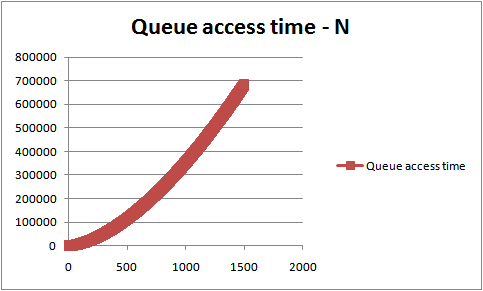
\includegraphics[scale=0.5]{img/big-O-1q.eps}
        \caption{Queue access count v.s. $n$.} \label{fig:big-O-1q}
       \end{center}
\end{figure}

The C program based on this algorithm takes only 0.016[s] to get the right answer
859963392. Which is 2500 times faster than the brute force solution.

%% Functional 1Q solution
Improvement 1 can also be considered in recursive way. Suppose $X$ is the infinity
series for all numbers which only contain factors of 2, 3, or 5. The following
formula shows an interesting relationship.

\be
  X = \{1\} \cup \{2x: \forall x \in X\} \cup \{3x: \forall x \in X \} \cup \{5x: \forall x \in X \}
\ee

Where we can define $\cup$ to a special form so that all elements are stored in order
as well as unique to each other. Suppose that $X=\{x_1, x_2, x_3...\}$, $Y=\{y_1, y_2, y_3, ...\}$, $X' = \{x_2, x_3, ...\}$ and $Y'=\{y_2, y_3, ...\}$. We have

\[
X \cup Y = \left \{
  \begin{array}{r@{\quad:\quad}l}
  X & Y = \phi \\
  Y & X = \phi \\
  \{ x_1, X' \cup Y \} & x_1 < y_1 \\
  \{ X' \cup Y' \} & x_1 = y_1 \\
  \{ y_1, X \cup Y' \} & x_1 > y_1
  \end{array}
\right.
\]

In a functional programming language such as Haskell, which supports 
lazy evaluation, The above infinity series functions can be translate
into the following program.

\lstset{language=Haskell}
\begin{lstlisting}
ns = 1:merge (map (*2) ns) (merge (map (*3) ns) (map (*5) ns))

merge [] l = l
merge l [] = l
merge (x:xs) (y:ys) | x <y = x : merge xs (y:ys)
                    | x ==y = x : merge xs ys
                    | otherwise = y : merge (x:xs) ys
\end{lstlisting}

By evaluate ns !! (n-1), we can get the 1500th number as
below.

\begin{verbatim}
>ns !! (1500-1)
859963392
\end{verbatim}

\subsection{Improvement 2}
Considering the above solution, although it is much faster than the brute-force one,
It still has some drawbacks. It produces many duplicated numbers and they are
finally dropped when examine the queue. Secondly, it does linear scan and insertion
to keep the order of all elements in the queue, which degrade the ENQUEUE operation
from $O(1)$ to $O(|Q|)$.

If we use three queues instead of using only one, we can improve the solution one
step ahead. Denote these queues as $Q_2$, $Q_3$, and $Q_5$, and we initialize
them as $Q_2=\{ 2 \}$, $Q_3 = \{ 3\}$ and $Q_5 = \{ 5 \}$. Each time we DEQUEUEed
the smallest one from $Q_2$, $Q_3$, and $Q_5$ as $x$. And do the following test:

\begin{itemize}
\item If $x$ comes from $Q_2$, we ENQUEUE $2x$, $3x$, and $5x$ back to 
$Q_2$, $Q_3$, and $Q_5$ respectively;
\item If $x$ comes from $Q_3$, we only need ENQUEUE $3x$ to $Q_3$, and $5x$ to $Q_5$;
We needn't ENQUEUE $2x$ to $Q_2$, because $2x$ have already existed in $Q_3$;
\item If $x$ comes from $Q_5$, we only need ENQUEUE $5x$ to $Q_5$; there is
no need to ENQUEUE $3x$, $5x$ to $Q_3$, $Q_5$ because they have already been
in the queues;
\end{itemize}

We repeatedly ENQUEUE the smallest one until we find the $n$-th element.

\begin{figure}[htbp]
       \begin{center}
       	  \includegraphics[scale=0.5]{img/q235-1.ps}
       	  \includegraphics[scale=0.5]{img/q235-2.ps}
       	  \includegraphics[scale=0.5]{img/q235-3.ps}
       	  \includegraphics[scale=0.5]{img/q235-4.ps}
        \caption{First 4 steps of constructing numbers with $Q_2$, $Q_3$, and $Q_5$. \newline
        1. Queues are initialized with 2, 3, 5 as the only element;\newline
        2. New elements 4, 6, and 10 are pushed back; \newline
        3. New elements 9, and 15, are pushed back; \newline
        4. New elements 8, 12, and 20 are pushed back; \newline
        5. New element 25 is pushed back.} \label{fig:q235}
       \end{center}
\end{figure}

The algorithm based on this idea is implemented as below.

\begin{algorithmic}[1]
\Function{Get-Number}{$n$}
  \If{$n = 1$}
    \State \Return $1$
  \Else
    \State $Q_2 \gets \{ 2 \}$
    \State $Q_3 \gets \{ 3 \}$
    \State $Q_5 \gets \{ 5 \}$
    \While{$n > 1$}
      \State $x \gets min($\Call{Head}{$Q_2$}, \Call{Head}{$Q_3$}, \Call{Head}{$Q_5$}$)$
      \If{$x = $ \Call{Head}{$Q_2$}}
        \State \Call{Dequeue}{$Q_2$}
        \State \Call{Enqueue}{$Q_2, 2x$}
        \State \Call{Enqueue}{$Q_3, 3x$}
        \State \Call{Enqueue}{$Q_5, 5x$}
      \ElsIf{$x=$ \Call{Head}{$Q_3$}}
        \State \Call{Dequeue}{$Q_3$}
        \State \Call{Enqueue}{$Q_3, 3x$}
        \State \Call{Enqueue}{$Q_5, 5x$}
      \Else
        \State \Call{Dequeue}{$Q_5$}
        \State \Call{Enqueue}{$Q_5, 5x$}
      \EndIf
      \State $n \gets n - 1$
    \EndWhile
    \State \Return $x$
  \EndIf
\EndFunction
\end{algorithmic}

This algorithm loops $n$ times, and within each loop, it extract one head
element from the three queues, which takes constant time. Then it appends
one to three new elements at the end of queues which bounds to constant time
too. So the total time of the algorithm bounds to $O(n)$. The C++ program
translated from this algorithm shown below takes less than 1 $\mu$s to 
produce the 1500th number, 859963392.

\lstset{language=C++}
\begin{lstlisting}
typedef unsigned long Integer;

Integer get_number(int n){
  if(n==1) 
    return 1;
  queue<Integer> Q2, Q3, Q5;
  Q2.push(2);
  Q3.push(3);
  Q5.push(5);
  Integer x;
  while(n-- > 1){
    x = min(min(Q2.front(), Q3.front()), Q5.front());
    if(x==Q2.front()){
      Q2.pop();
      Q2.push(x*2);
      Q3.push(x*3);
      Q5.push(x*5);
    }
    else if(x==Q3.front()){
      Q3.pop();
      Q3.push(x*3);
      Q5.push(x*5);
    }
    else{
      Q5.pop();
      Q5.push(x*5);
    }
  }
  return x;
}
\end{lstlisting}

This solution can be also implemented in Functional way. We define
a function $take(n)$, which will return the first $n$ numbers contains
only factor 2, 3, or 5.

\[
  take(n) = f(n, \{1\}, \{2\}, \{3\}, \{5\})
\]
Where
\[
 f(n, X, Q_2, Q_3, Q_5) = \left \{
  \begin{array}{r@{\quad:\quad}l}
  X & n = 1 \\
  f(n-1, X \cup \{x\}, Q_2', Q_3', Q_5') & otherwise
  \end{array}
\right.
\]

\[
 x = min(Q_{21}, Q_{31}, Q_{51})
\]
\[
 Q_2', Q_3', Q_5' = \left \{
 \begin{array}{r@{\quad:\quad}l}
 \{Q_{22}, Q_{23}, ...\} \cup \{2x\}, Q_3 \cup \{3x\}, Q_5 \cup \{5x\} & x = Q_{21} \\
 Q_2, \{Q_{32}, Q_{33}, ...\} \cup \{3x\}, Q5 \cup \{5x\} & x = Q_{31} \\
 Q_2, Q_3, \{Q_{52}, Q_{53}, ...\} \cup \{5x\} & x = Q_{51}
 \end{array}
 \right.
\]

And these functional definition can be realized in Haskell as the following.

\lstset{language=Haskell}
\begin{lstlisting}
ks 1 xs _ = xs
ks n xs (q2, q3, q5) = ks (n-1) (xs++[x]) update
    where 
      x = minimum $ map head [q2, q3, q5]
      update | x == head q2 = ((tail q2)++[x*2], q3++[x*3], q5++[x*5])
             | x == head q3 = (q2, (tail q3)++[x*3], q5++[x*5])
             | otherwise = (q2, q3, (tail q5)++[x*5])

takeN n = ks n [1] ([2], [3], [5])
\end{lstlisting} %$

Invoke `last takeN 1500' will generate the correct answer 859963392.

% ================================================================
%                 Short summary
% ================================================================
\section{Notes and short summary}
If review the 2 puzzles, we found in both cases, the brute-force solutions
are so weak. In the first problem, it's quite poor in dealing with
long ID list, while in the second problem, it doesn't work at all.

The first problem shows the power of algorithms, while the second 
problem tells why data structure is important. There are plenty
of interesting problems, which are hard to solve before computer
was invented. With the aid of computer and programming, we are able
to find the answer in a quite different way. Compare to what we 
learned in mathematics course in school, we haven't been taught the method 
like this. 

While there have been already a lot of wonderful books about
algorithms, data structures and math, however, few of them 
provide the comparison between the procedural solution and 
the functional solution. From the above discussion, it can be 
found that functional solution sometimes is very expressive 
and they are close to what we are familiar in mathematics.

This series of post focus on providing both imperative and functional
algorithms and data structures. Many functional data structures
can be referenced from Okasaki's book\cite{okasaki-book}. While
the imperative ones can be founded in classic text books \cite{CLRS}
or even in WIKIpedia.
Multiple
programming languages, including, C, C++, Python, Haskell, and
Scheme/Lisp will be used. In order to make it easy to read
by programmers with different background, pseudo code and mathematical
function are the regular descriptions of each post.

The author is NOT a native English speaker, the reason why 
this book is only available in English for the time being
is because the contents are still changing frequently. Any
feedback, comments, or criticizes are welcome.

\section{Structure of the contents}
In the following series of post, I'll first introduce about
elementary data structures before algorithms, because many
algorithms need knowledge of data structures as prerequisite.

The `hello world' data structure, binary search tree is the
first topic; Then we introduce how to solve the balance problem
of binary search tree. After that, I'll show other interesting
trees. Trie, Patricia, suffix trees are useful in text manipulation.
While B-trees are commonly used in file system and data base
implementation.

The second part of data structures is about heaps. We'll
provide a general Heap definition and introduce about binary
heaps by array and by explicit binary trees. Then we'll
extend to K-ary heaps including Binomial heaps, Fibonacci
heaps, and pairing heaps.

Array and queues are considered among the easiest data structures
typically, However, we'll show how difficult to implement 
them in the third part.

As the elementary sort algorithms, we'll introduce insertion
sort, quick sort, merge sort etc in both imperative way
and functional way.

The final part is about searching, besides the element
searching, we'll also show string matching algorithms
such as KMP.

All the posts are provided under GNU FDL (Free document
license), and programs are under GNU GPL.

% ================================================================
%                 Appendix
% ================================================================
\section{Appendix} \label{appendix}
%\appendix
All programs provided along with this article are free for
downloading. download position: 
  http://sites.google.com/site/algoxy/introduction

\begin{thebibliography}{99}

\bibitem{Bird-book}
Richard Bird. ``Pearls of functional algorithm design''. Cambridge University Press; 1 edition (November 1, 2010). ISBN-10: 0521513383

\bibitem{Bentley}
Jon Bentley. ``Programming Pearls(2nd Edition)''. Addison-Wesley Professional; 2 edition (October 7, 1999). ISBN-13: 978-0201657883

\bibitem{okasaki-book}
Chris Okasaki. ``Purely Functional Data Structures''. Cambridge university press, (July 1, 1999), ISBN-13: 978-0521663502

\bibitem{CLRS}
Thomas H. Cormen, Charles E. Leiserson, Ronald L. Rivest and Clifford Stein. ``Introduction to Algorithms, Second Edition''. The MIT Press, 2001. ISBN: 0262032937.

\end{thebibliography}

\ifx\wholebook\relax \else
\end{document}
\fi
